%%%%%%%%%%%%%%%%%%%%%%%%%%%%%%%%%%%%%%%%%%%%%%%%%%
%%%%%%%%%%%%%%%%%%%%%%%%%%%%%%%%%%%%%%%%%%%%%%%%%%
%%%%%%%%%%%%%%%%%%%%%%%%%%%%%%%%%%%%%%%%%%%%%%%%%%
\documentclass[11pt]{article}

\usepackage{amsmath, amsthm, amssymb}
\usepackage{enumerate}
\usepackage{pdflscape}
\usepackage{caption}
\usepackage{bm}

\usepackage{ifpdf}
\ifpdf
\usepackage[pdftex]{graphicx}
\else
\usepackage[dvips]{graphicx}
\fi
\usepackage{tikz}
 	 \usetikzlibrary{arrows,backgrounds}
\usepackage[all]{xy}

\usepackage{multicol}

\usepackage{tocvsec2}

\usepackage{bbm}

\input xy
\xyoption{all}

\usepackage[pdftex,plainpages=false,hypertexnames=false,pdfpagelabels]{hyperref}
\newcommand{\arxiv}[1]{\href{http://arxiv.org/abs/#1}{\tt arXiv:\nolinkurl{#1}}}
\newcommand{\arXiv}[1]{\href{http://arxiv.org/abs/#1}{\tt arXiv:\nolinkurl{#1}}}
\newcommand{\doi}[1]{\href{http://dx.doi.org/#1}{{\tt DOI:#1}}}
\newcommand{\euclid}[1]{\href{http://projecteuclid.org/getRecord?id=#1}{{\tt #1}}}
\newcommand{\mathscinet}[1]{\href{http://www.ams.org/mathscinet-getitem?mr=#1}{\tt #1}}
\newcommand{\googlebooks}[1]{(preview at \href{http://books.google.com/books?id=#1}{google books})}
\newcommand{\Ws}{\text{W*}}

\usepackage{xcolor}
\definecolor{dark-red}{rgb}{0.7,0.25,0.25}
\definecolor{dark-blue}{rgb}{0.15,0.15,0.55}
\definecolor{medium-blue}{rgb}{0,0,.8}
\definecolor{DarkGreen}{RGB}{0,150,0}
\definecolor{DarkPurple}{RGB}{148,0,211}
\definecolor{DarkYellow}{RGB}{255,230,0}
\definecolor{rho}{named}{red}
\hypersetup{
   colorlinks, linkcolor={purple},
   citecolor={medium-blue}, urlcolor={medium-blue}
}

%\addtolength{\textwidth}{.5in}
\usepackage{longtable}
\usepackage{fullpage}
%\renewcommand{\arraystretch}{1.5}

% Page size %%%%%%%%%%%%%%%%%%%%%%%%%%%%%%%%%%%%%%%%%%%
\setlength\topmargin{-.25in}
\setlength\headheight{0in}
\setlength\headsep{.2in}
\setlength\textheight{9in}
%\addtolength{\hoffset}{-0.25in}
%\addtolength{\textwidth}{.5in}
\setlength\parindent{0.25in}

% Theorems %%%%%%%%%%%%%%%%%%%%%%%%%%%%%%%%%%%%%%%%%%
\theoremstyle{plain}
\newtheorem{thm}{Theorem}[section]
\newtheorem*{thm*}{Theorem}
\newtheorem{thmalpha}{Theorem}
\renewcommand*{\thethmalpha}{\Alph{thmalpha}}
\newtheorem{cor}[thm]{Corollary}
\newtheorem{coralpha}[thmalpha]{Corollary}
\newtheorem*{cor*}{Corollary}
\newtheorem{conj}[thm]{Conjecture}
\newtheorem{conjalpha}[thmalpha]{Conjecture}
\newtheorem*{conj*}{Conjecture}
\newtheorem{lem}[thm]{Lemma}
\newtheorem{fact}[thm]{Fact}
\newtheorem{facts}[thm]{Facts}
\newtheorem{prop}[thm]{Proposition}
\newtheorem{question}[thm]{Question}
\newtheorem*{quest*}{Question}
\newtheorem*{claim*}{Claim}
\newtheorem{quests}[thm]{Questions}
\theoremstyle{definition}
\newtheorem{defn}[thm]{Definition}
\newtheorem{construction}[thm]{Construction}
\newtheorem{alg}[thm]{Algorithm}
\newtheorem{assumption}[thm]{Assumption}
\newtheorem{nota}[thm]{Notation}
\newtheorem{nb}[thm]{Note}
\newtheorem{note}[thm]{Note}
\newtheorem{exs}[thm]{Examples}
\newtheorem{ex}[thm]{Example}
\newtheorem{example}[thm]{Example}
\newtheorem{exercise}[thm]{Exercise}
\newtheorem{sub-ex}[thm]{Sub-Example}
\newtheorem{rem}[thm]{Remark}
\newtheorem*{rem*}{Remark}
\newtheorem{remark}[thm]{Remark}
\newtheorem{rems}[thm]{Remarks}
\newtheorem{warn}[thm]{Warning}

% Operators %%%%%%%%%%%%%%%%%%%%%%%%%%%%%%%%%%%%%%%%%%%
\DeclareMathOperator{\Ad}{Ad}
\DeclareMathOperator{\Aut}{Aut}
\DeclareMathOperator{\coev}{coev}
\DeclareMathOperator{\Dim}{Dim}
\DeclareMathOperator{\Dom}{Dom}
\DeclareMathOperator{\End}{End}
\DeclareMathOperator{\ev}{ev}
\DeclareMathOperator{\gr}{gr}
\DeclareMathOperator{\Hom}{Hom}
\DeclareMathOperator{\Mat}{Mat}
\DeclareMathOperator{\Mor}{Mor}
\DeclareMathOperator{\op}{op}
\DeclareMathOperator{\ONB}{ONB}
\DeclareMathOperator{\Ob}{Ob}
\DeclareMathOperator{\rev}{rev}
\DeclareMathOperator{\spann}{span}
\DeclareMathOperator{\supp}{supp}
\DeclareMathOperator{\id}{id}
\DeclareMathOperator{\Isom}{Isom}
\DeclareMathOperator{\ind}{ind}
\DeclareMathOperator{\im}{im}
\DeclareMathOperator{\Irr}{Irr}
\DeclareMathOperator{\Spec}{Spec}
\DeclareMathOperator{\Stab}{Stab}
\DeclareMathOperator{\Tr}{Tr}
\DeclareMathOperator{\tr}{tr}
\DeclareMathOperator{\Tube}{Tube}
\DeclareMathOperator{\Gr}{Gr}


% Math %%%%%%%%%%%%%%%%%%%%%%%%%%%%%%%%%%%%%%%%%%%%%
\newcommand{\D}{\displaystyle}
\newcommand{\comment}[1]{}
\newcommand{\hs}{\hspace{.07in}}
\newcommand{\hsp}[1]{\hs\text{#1}\hs}
\newcommand{\be}{\begin{enumerate}[label=(\arabic*)]}
\newcommand{\ee}{\end{enumerate}}
\newcommand{\itm}[1]{\item[\underline{\ensuremath{#1}:}]}
\newcommand{\itt}[1]{\item[\underline{\text{#1}:}]}
\newcommand{\N}{\mathbb{N}}
\newcommand{\Natural}{\mathbb{N}}
\newcommand{\Z}{\mathbb{Z}}
\newcommand{\Q}{\mathbb{Q}}
\newcommand{\F}{\mathbb{F}}
\newcommand{\R}{\mathbb{R}}
\newcommand{\C}{\mathbb{C}}
\newcommand{\B}{\mathbb{B}}
\renewcommand{\P}{\mathbb{P}}
\newcommand{\I}{\infty}
\newcommand{\set}[2]{\left\{#1 \middle| #2\right\}}
\newcommand{\thh}{^{\text{th}}}
\renewcommand{\a}{\mathfrak{a}}
\renewcommand{\b}{\mathfrak{b}}
\renewcommand{\c}{\mathfrak{c}}
\newcommand{\n}{\mathfrak{n}}
\newcommand{\m}{\mathfrak{m}}
\newcommand{\bbOne}{\mathbbm{1}}
\renewcommand{\alg}[1]{{\bm{\langle} #1\bm{\rangle}}}

\newcommand{\dave}[1]{\marginpar{\tiny \textcolor{orange}{DP: #1}}}
\newcommand{\corey}[1]{\marginpar{\tiny \textcolor{green}{CJ: #1}}}
\newcommand{\Af}{\mathcal{A}\Lambda_{F}}
\newcommand{\WStar}{\bfW\text{*}}
%\newcommand{\Irr}{\text{Irr}(\mathcal{C})}

% tricky way to iterate macros over a list
\def\semicolon{;}
\def\applytolist#1{
    \expandafter\def\csname multi#1\endcsname##1{
        \def\multiack{##1}\ifx\multiack\semicolon
            \def\next{\relax}
        \else
            \csname #1\endcsname{##1}
            \def\next{\csname multi#1\endcsname}
        \fi
        \next}
    \csname multi#1\endcsname}

% \def\cA{{\cal A}} for A..Z
\def\calc#1{\expandafter\def\csname c#1\endcsname{{\mathcal #1}}}
\applytolist{calc}QWERTYUIOPLKJHGFDSAZXCVBNM;
% \def\bbA{{\mathbb A}} for A..Z
\def\bbc#1{\expandafter\def\csname bb#1\endcsname{{\mathbb #1}}}
\applytolist{bbc}QWERTYUIOPLKJHGFDSAZXCVBNM;
% \def\bfA{{\mathbf A}} for A..Z
\def\bfc#1{\expandafter\def\csname bf#1\endcsname{{\mathbf #1}}}
\applytolist{bfc}QWERTYUIOPLKJHGFDSAZXCVBNM;
% \def\sA{{\sf A}} for A..Z
\def\sfc#1{\expandafter\def\csname s#1\endcsname{{\sf #1}}}
\applytolist{sfc}QWERTYUIOPLKJHGFDSAZXCVBNM;
% \def\fA{{\mathfrak A}} for A..Z
\def\fc#1{\expandafter\def\csname f#1\endcsname{{\mathfrak #1}}}
\applytolist{fc}QWERTYUIOPLKJHGFDSAZXCVBNM;


\newcommand{\PA}{\cP\hspace{-.1cm}\cA}
\newcommand{\Fun}{{\sf Fun}}
\newcommand{\Rep}{{\sf Rep}}
\newcommand{\Set}{{\sf Set}}
\newcommand{\FreeMod}{{\sf FreeMod}}
\newcommand{\Mod}{{\sf Mod}}
\newcommand{\Proj}{{\sf Proj}}
\newcommand{\AlgBim}{{\sf AlgBim}}
\newcommand{\Bimod}{{\sf Bimod}}
\newcommand{\Bim}{{\sf Bim}}
\newcommand{\bfBim}{{\sf Bim_{bf}}}
\newcommand{\spBim}{{\sf Bim^{sp}}}
\newcommand{\spbfBim}{{\sf Bim_{bf}^{sp}}}
\renewcommand{\Vec}{{\sf Vec}}
\newcommand{\fdVec}{{\sf Vec_{fd}}}
\newcommand{\Hilb}{{\sf Hilb}}
\newcommand{\fdHilb}{{\sf Hilb_{fd}}}
\newcommand{\ConAlg}{{\sf ConAlg}}
\newcommand{\DisInc}{{\sf DisInc}}


\newcommand{\jw}[1]{f^{(#1)}}
\newcommand{\todo}[1]{\textcolor{blue}{\textbf{TODO: #1}}}
\newcommand{\nn}[1]{\textcolor{red}{[[#1]]}}
\newcommand{\noshow}[1]{}
\newcommand{\MR}[1]{}
\newcommand{\TL}{\cT\hspace{-.08cm}\cL}
\newcommand{\rhoE}{\textcolor{rho}{e_1}}
\newcommand{\rhoJW}{\textcolor{rho}{\jw{2}}}
\newcommand{\Cstar}{{\rm C^*}}

% TikZ operators %%%%%%%%%%%%%%%%%%%%%%%%%%%%%%%%%%%%%%%%
\usetikzlibrary{shapes}
\usetikzlibrary{cd}
\usetikzlibrary{backgrounds}
\usetikzlibrary{decorations,decorations.pathreplacing,decorations.markings}
\usetikzlibrary{fit,calc,through}
\usetikzlibrary{external}
\usetikzlibrary{arrows}
\tikzset{vertex/.style = {shape=circle,draw,fill=black,inner sep=0pt,minimum size=5pt}}
\tikzset{edge/.style = {->,> = latex', bend right}}
\tikzset{
	super thick/.style={line width=3pt}
}
\tikzset{
    quadruple/.style args={[#1] in [#2] in [#3] in [#4]}{
        #1,preaction={preaction={preaction={draw,#4},draw,#3}, draw,#2}
    }
}
\tikzstyle{shaded}=[fill=red!10!blue!20!gray!30!white]
\tikzstyle{unshaded}=[fill=white]
\tikzstyle{empty box}=[circle, draw, thick, fill=white, opaque, inner sep=2mm]
\tikzstyle{annular}=[scale=.7, inner sep=1mm, baseline]
\tikzstyle{rectangular}=[scale=.75, inner sep=1mm, baseline=-.1cm]
\tikzstyle{mid>}=[decoration={markings, mark=at position 0.5 with {\arrow{>}}}, postaction={decorate}]
\tikzstyle{mid<}=[decoration={markings, mark=at position 0.5 with {\arrow{<}}}, postaction={decorate}]
\tikzstyle{over}=[double, draw=white, super thick, double=]
\tikzstyle{box} = [rectangle,draw,rounded corners=5pt,very thick]

% macros for pictures %%%%%%%%%%%%%%%%%%%%%%%%%%%%%%%%%%%%%%%

\newcommand{\roundNbox}[6]{
	\draw[rounded corners=5pt, very thick, #1] ($#2+(-#3,-#3)+(-#4,0)$) rectangle ($#2+(#3,#3)+(#5,0)$);
	\coordinate (ZZa) at ($#2+(-#4,0)$);
	\coordinate (ZZb) at ($#2+(#5,0)$);
	\node at ($1/2*(ZZa)+1/2*(ZZb)$) {#6};
}


\newcommand{\nbox}[6]{
	\draw[thick, #1] ($#2+(-#3,-#3)+(-#4,0)$) rectangle ($#2+(#3,#3)+(#5,0)$);
	\coordinate (ZZa) at ($#2+(-#4,0)$);
	\coordinate (ZZb) at ($#2+(#5,0)$);
	\node at ($1/2*(ZZa)+1/2*(ZZb)$) {#6};
}

\newcommand{\ncircle}[4]{
	\draw[very thick, #1] #2 circle (#3);
	\node at #2 {#4};
}

  \newcommand{\tikzmath}[2][]
     {\vcenter{\hbox{\begin{tikzpicture}[#1]#2
                     \end{tikzpicture}}}
     }

\newcommand{\halfDottedEllipse}[3]{
	\draw[thick] #1 arc(-180:0:{#2} and {#3});
	\draw[thick, dotted] ($ #1 + 2*(#2,0)$) arc(0:180:{#2} and {#3});
}

\newcommand{\downTube}[1]{
	\draw[thick, unshaded] #1 -- ($#1 + (0,-.4)$) ;
	\halfDottedEllipse{($#1 + (0,-.4)$)}{.2}{.1}
	\draw[thick, unshaded] ($#1 + (.4,0)$) -- ($#1 + (.4,-.4)$);
}

\newcommand{\topPairOfPants}[2]{
	%pair of pants:
	\draw[thick] #1 .. controls ++(90:1cm) and ++(270:1cm) .. ($ #1 + (.75,2) $);
	\draw[thick] ($ #1 + (2.5,0) $) .. controls ++(90:1cm) and ++(270:1cm) .. ($ #1 + (1.75,2) $);
	\draw[thick] ($ #1 + (1,0) $).. controls ++(90:1cm) and ++(90:1cm) .. ($ #1 + (1.5,0) $); 
	\draw[thick] ($ #1 + (1.25,2) $) ellipse (.5cm and .2cm);
	\halfDottedEllipse{#1}{.5}{.2}
	\halfDottedEllipse{($ #1 + (1.5,0) $)}{.5}{.2}

}

% colors %%%%%%%%%%%%%%%%%%%%%%%%%%%%%%%%%%%%%%%%
\newcommand{\cupcolor}{DarkGreen}
\newcommand{\alphacolor}{blue}
\newcommand{\betacolor}{red}

\begin{document}
\title{The enriched tube algebra}
\author{Peter Huston, Corey Jones, and David Penneys}
\date{\today}
\maketitle
\begin{abstract}
%This is the submitted version of \arxiv{???}.
\end{abstract}

%%%%%%%%%%%%%%%%%%%%%%%%%%%%%%%%%%%%%%%%%%%%%%%%%%%%%%%%%%%%%%%
%%%%%%%%%%%%%%%%%%%%%%%%%%%%%%%%%%%%%%%%%%%%%%%%%%%%%%%%%%%%%%%
%%%%%%%%%%%%%%%%%%%%%%%%%%%%%%%%%%%%%%%%%%%%%%%%%%%%%%%%%%%%%%%
\section{Definition of the enriched tube algebra}

Let $\cV$ be a unitary ribbon fusion category.
Suppose $\cC$ is a \emph{module tensor category} over $\cV$, i.e.,
$\cC$ is a unitary tensor category with its canonical spherical structure, and $\Phi^{\scriptscriptstyle\cZ} : \cV \to \cZ(\cC)$ is a pivotal dagger tensor functor.
Letting $F: \cZ(\cC) \to \cC$ be the forgetful functor, $\Phi:=F\circ \Phi^{\scriptscriptstyle\cZ}$ admits a right adjoint $\Tr_\cV : \cC \to \cV$ called the \emph{categorified trace} \cite{MR3578212}.
$$
\begin{tikzcd}
\cV
\ar[]{rr}{\Phi^{\scriptscriptstyle\cZ}}
\ar[shift left]{drr}{\Phi}
&&
\cZ(\cC)
\ar[]{d}{F}
\\
&&
\cC
\ar[shift left]{ull}{\Tr_\cV}
\end{tikzcd}
$$
Recall that the non-enriched tube algebra for $\cC$ is 
$$
\Tube(\cC)
:=
\bigoplus_{c,x,y\in\Irr(\cC)}
\cC(c\otimes x \to y\otimes c)
$$
with multiplication given for $f\in \cC(c\otimes x \to y\otimes c)$ and $g\in \cC(d\otimes y \to z\otimes d)$ by
\begin{equation}
\label{eq:MultiplicationInTubeAlgebra}
g\cdot f
:=
\sum_{\substack{
b\in \Irr(\cC)
\\
\alpha\in \Isom(d\otimes c \to b)
}}
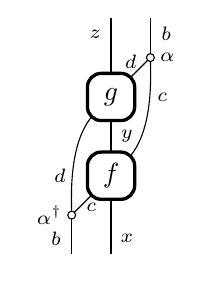
\begin{tikzpicture}[baseline=-.1cm]
	\draw (0,-1.5) -- (0,1.5);
	\draw (0,.5) -- (-.2,.3) .. controls ++(225:.5cm) and ++(90:.2cm) .. (-.5,-1);
	\draw (0,-.5) -- (-.5,-1);
	\draw (-.5,-1) -- (-.5,-1.5);
	\filldraw[fill=white] (-.5,-1) circle (.05cm) node [left] {\scriptsize{$\alpha^\dag$}};
	\draw (0,-.5) -- (.2,-.3) .. controls ++(45:.5cm) and ++(-90:.2cm) .. (.5,1);
	\draw (0,.5) -- (.5,1);
	\draw (.5,1) -- (.5,1.5);
	\filldraw[fill=white] (.5,1) circle (.05cm) node [right] {\scriptsize{$\alpha$}};
	\roundNbox{unshaded}{(0,-.5)}{.3}{0}{0}{$f$}
	\roundNbox{unshaded}{(0,.5)}{.3}{0}{0}{$g$}
	\node at (-.7,-1.3) {\scriptsize{$b$}};
	\node at (.2,-1.3) {\scriptsize{$x$}};
	\node at (-.25,-.9) {\scriptsize{$c$}};
	\node at (-.65,-.5) {\scriptsize{$d$}};
	\node at (.2,0) {\scriptsize{$y$}};
	\node at (.65,.5) {\scriptsize{$c$}};
	\node at (.25,.95) {\scriptsize{$d$}};
	\node at (-.2,1.3) {\scriptsize{$z$}};
	\node at (.7,1.3) {\scriptsize{$b$}};
\end{tikzpicture}
\end{equation}
where for $a,b,c\in \Irr(\cC)$, $\Isom(a\otimes b \to c)$ is a choice of orthonormal basis for $\cC(a\otimes b \to c)$ under the inner product $\langle  \eta, \xi \rangle_{\Isom} := \eta \circ \xi^*$.
Observe that since we are summing over $\alpha$ and $\overline{\alpha}$ in \eqref{eq:MultiplicationInTubeAlgebra}, this sum is independent of the choice of orthonormal basis, and this independence is crucial to proving associativity of multiplication.
The $*$-algebra structure on $\Tube(\cC)$ is given on $f\in \cC(c\otimes x \to y\otimes c)$ by
\begin{equation}
\label{eq:TubeAlgebraStarStructure}
f^*:=
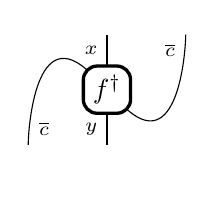
\begin{tikzpicture}[baseline=-.1cm]
	\draw (0,-.7) -- (0,.7);
	\draw (0,0) -- (.2,-.2) .. controls ++(-45:1cm) and ++(-90:.2cm) .. (1,.7);
	\draw (0,0) -- (-.2,.2) .. controls ++(135:1cm) and ++(90:.2cm) .. (-1,-.7);
	\roundNbox{unshaded}{(0,0)}{.3}{0}{0}{$f^\dag$}
	\node at (-.2,.5) {\scriptsize{$x$}};
	\node at (-.2,-.5) {\scriptsize{$y$}};
	\node at (.8,.5) {\scriptsize{$\overline{c}$}};
	\node at (-.8,-.5) {\scriptsize{$\overline{c}$}};
\end{tikzpicture}
\in
\cC(\overline{c}\otimes y \to x\otimes \overline{c}).
\end{equation}

In the enriched setting, since 
$$
\cC(c\otimes x \to y\otimes c)
\cong
\cC(1_\cC \to y \otimes c\otimes \overline{x}\otimes \overline{c}) 
\cong 
\Tr_\cV(y\otimes c\otimes \overline{x}\otimes \overline{c}),
$$
we define the $\cV$-\emph{enriched tube algebra object}
$$
\Tube_\cV(\cC)
:=
\bigoplus_{c,x,y\in\Irr(\cC)}
\Tr_\cV(y\otimes c\otimes \overline{x}\otimes \overline{c})
\in \cV
$$
with multiplication $\Tube_\cV(\cC) \otimes \Tube_\cV(\cC) \to \Tube_\cV(\cC)$ given by
\begin{equation}
\label{eq:EnrichedTubeAlgebraMultiplication}
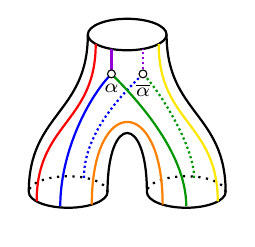
\begin{tikzpicture}[baseline=1cm]	
	\pgfmathsetmacro{\voffset}{.12};
	\pgfmathsetmacro{\hoffset}{.1};
	\pgfmathsetmacro{\hoffsetTop}{.2};
%
	\coordinate (a1) at (0,0);
	\coordinate (a2) at ($ (a1) + (1.5,0)$);
	\coordinate (b1) at ($ (a1) + (.75,1.5)$);
	\coordinate (c1) at ($ (a1) + (.75,2)$);
%
	\topPairOfPants{(0,0)}{}
%
%	%lower traciator
	\draw[thick, red] ($ (a1) + (\hoffset,0) + (0,-\voffset)$) .. controls ++(90:1cm) and ++(270:1cm) .. ($ (c1) + 1*(\hoffset,0) + (0,-\voffset) $);
	\draw[thick, DarkYellow] ($ (a2) + 9*(\hoffset,0) + (0,-\voffset)$) .. controls ++(90:1cm) and ++(270:1cm) .. ($ (c1) + 9*(\hoffset,0) + (0,-\voffset) $);
	\draw[thick, orange] ($ (a1) + 8*(\hoffset,0) + (0,-.16)$) .. controls ++(90:1.4cm) and ++(90:1.4cm) .. ($ (a2) + 2*(\hoffset,0) + (0,-.16) $);
	\draw[thick, blue] ($ (a1) + 4*(\hoffset,0) + (0,-.18)$) .. controls ++(90:.7cm) and ++(225:.4cm) .. ($ (b1) + 3*(\hoffset,0) $);		
	\draw[thick, blue, densely dotted] ($ (a1) + 7*(\hoffset,0) + (0,.18)$) .. controls ++(90:.6cm) and ++(225:.3cm) .. ($ (b1) + 7*(\hoffset,0) $);
	\draw[thick, DarkGreen] ($ (a2) + 5*(\hoffset,0) + (0,-.18)$) .. controls ++(90:.7cm) and ++(-45:.4cm) .. ($ (b1) + 3*(\hoffset,0) $);		
	\draw[thick, DarkGreen, densely dotted] ($ (a2) + 6*(\hoffset,0) + (0,.18)$) .. controls ++(90:.4cm) and ++(-45:.3cm) .. ($ (b1) + 7*(\hoffset,0) $);		
	\draw[thick, DarkPurple] ($ (b1) + 3*(\hoffset,0) $) -- ($ (c1) + 3*(\hoffset,0) + (0,-.18) $);		
	\draw[thick, DarkPurple, densely dotted] ($ (b1) + 7*(\hoffset,0) $) -- ($ (c1) + 7*(\hoffset,0) + (0,-.18) $);		
	\filldraw[fill=white] ($ (b1) + 3*(\hoffset,0) $) circle (.05cm) node [below] {\scriptsize{$\alpha$}};
	\filldraw[fill=white] ($ (b1) + 7*(\hoffset,0) $) circle (.05cm) node [below] {\scriptsize{$\overline{\alpha}$}};
\end{tikzpicture}
:=
{\begin{split}
\Tr_\cV(
\id_z\otimes \alpha \otimes \id_{x} \otimes \overline{\alpha}
)
&\circ
\tau^{-1}_{\overline{d}, z\otimes d\otimes \overline{y} \otimes y\otimes c \otimes \overline{x}\otimes \overline{c}}
\\&\circ
\mu_{\overline{d}\otimes z\otimes d\otimes \overline{y} , y\otimes c \otimes \overline{x}\otimes \overline{c}}
\circ
(
\tau_{z\otimes d\otimes \overline{y}, \overline{d}} 
\otimes 
\id_{y \otimes c\otimes \overline{x}\otimes \overline{c}}
)
\end{split}}
\end{equation}
Here we use the graphical notation of strings on the backs of tubes following \cite[Rem.~4.20]{MR3578212}.

We now define a $*$-structure on $\Tube_\cV(\cC)$ via an involutive algebra isomorphism $\sigma: \Tube_\cV(\cC) \to \overline{\Tube_\cV(\cC)}$ such that $\overline{\sigma}\circ \sigma = \id_{\Tube_\cV(\cC)}$ (here we suppress $\varphi_{\Tube_\cV(\cC)}$) \cite[Prop.~3.19]{MR3687214}.
Since $(\overline{\,\cdot\,},\nu,\varphi,r)$ is an involutive anti-linear anti-tensor $\dag$-functor and $\Tr_\cV$ is \emph{involutive} \cite{uAPA} with coherence unitary isomorphisms $\chi_c : \Tr_\cV(\overline{c}) \to \overline{\Tr_\cV(c)}$, we define $\sigma$ component-wise by
$$
\sigma_{c,x,y}:= 
\Tr_\cV(y\otimes c\otimes \overline{x}\otimes \overline{c})
\to
\overline{\Tr_\cV(x\otimes \overline{c}\otimes \overline{y}\otimes c)}
$$
is the composite
\begin{align*}
\Tr_\cV(y\otimes c\otimes \overline{x}\otimes \overline{c})
\cong
%&\xrightarrow{\Tr_\cV(\varphi_{y\otimes c\otimes \overline{x}\otimes \overline{c}})}
\Tr_\cV\left(\overline{\overline{y\otimes c\otimes \overline{x}\otimes \overline{c}}}\right)
%\\
&\xrightarrow{\chi_{\overline{y\otimes c\otimes \overline{x}\otimes \overline{c}}}}
\overline{\Tr_\cV\left(\overline{y\otimes c\otimes \overline{x}\otimes \overline{c}}\right)}
%\\&
%\xrightarrow{\cong}
\cong
\overline{\Tr_\cV\left(c\otimes \overline{y}\otimes \overline{c}\otimes x\right)}
\\&\xrightarrow{\overline{\tau^{-1}_{c, x\otimes \overline{c}\otimes \overline{y}}}}
\overline{\Tr_\cV\left(\overline{y}\otimes \overline{c}\otimes x\otimes c\right)}
\end{align*}
where we suppress all coherence isomorphisms $\nu,\varphi$ for $\overline{\,\cdot\,}$.

\begin{lem}
$\Tube_\cV(\cC)$ is a $*$-algebra object in $\cV$.
\end{lem}
\begin{proof}
That $\Tube_\cV(\cC)$ is an algebra object uses that the graphical calculus of strings on tubes is well-defined from \cite{1607.06041}, together with the fact that the tube algebra $\Tube(\cC)$ is an associative multiplication under \eqref{eq:MultiplicationInTubeAlgebra}.
One can also prove this directly using the relations in \cite{MR3578212} similar to the proof of Prop.~5.12 therein.
\nn{finish}
\end{proof}

\todo{
\begin{itemize}
\item
Show it's a $\Cstar$ algebra object.
(Note this is happening in $\cV^\natural$, which does not have a $\dag$-structure!)
\item
Define the enriched fusion of modules for $\Tube_\cV(\cC)$ over $\cZ_2(\cV)$, the M\"{u}ger center of $\cV$.
Make sure to reference \cite[\S5.3]{1709.01941}
\item
There should be a notion of an braided enriched monoidal category enriched over a symmetric monoidal category, and $\Rep(\Tube_\cV(\cC))$ should be an example of this.
\item
Show that $\Rep(\Tube_\cV(\cC))$ is $\cZ_2(\cV)$-braided monoidally equivalent to the enriched center of $\cC$ defined from \cite{1704.01447}.
\end{itemize}
}

%%%%%%%%%%%%%%%%%%%%%%%%%%%%%%%%%%%%%%%%%%%%%%%%%
\bibliographystyle{amsalpha}
{\footnotesize{
%\bibliography{../bibliography}
\bibliography{bibliography}
}}
\end{document}